\documentclass[12pt, letterpaper]{article}
\usepackage{graphicx}
\usepackage{caption}
\usepackage[hidelinks]{hyperref}
\usepackage{color}
\usepackage{listings}
\usepackage{array}
\usepackage{hhline}
\usepackage{multirow}
\graphicspath{{images/}}
\newcounter{nalg}[section] % defines algorithm counter for chapter-level
\renewcommand{\thenalg}{\thesection .\arabic{nalg}} %defines appearance of the algorithm counter
\DeclareCaptionLabelFormat{algocaption}{Algorithm \thenalg} % defines a new caption label as Algorithm x.y

\lstnewenvironment{algorithm}[1][] %defines the algorithm listing environment
{   
    \refstepcounter{nalg} %increments algorithm number
    \lstset{ %this is the stype
        mathescape=true,
        frame=tB,
        numbers=left, 
        numberstyle=\tiny,
        basicstyle=\scriptsize, 
        keywordstyle=\color{black}\bfseries\em,
        keywords={,input, output, return, datatype, function, in, if, else, foreach, while, begin, end, } %add the keywords you want, or load a language as Rubens explains in his comment above.
        numbers=left,
        xleftmargin=.04\textwidth,
        #1 % this is to add specific settings to an usage of this environment (for instnce, the caption and referable label)
    }
    \captionsetup{labelformat=algocaption,labelsep=colon} %defines the caption setup for: it ises label format as the declared caption label above and makes label and caption text to be separated by a ':'
}
{}
\begin{document}
    \begin{titlepage}
    \begin{center}
        \vspace*{1cm}
            
        \Huge
        \textbf{Final Report}
            
        \vspace{0.5cm}
        \LARGE
        Thermal Scanning App
            
        \vspace{1.5cm}
            
        \textbf{Colter Roche, Jose Bastardo}
            
        \vfill
          
        \Large
        Senior Design 1\\
        COP4934C.01\\
        \today
            
    \end{center}
\end{titlepage}
    \newpage
    \tableofcontents
    \newpage
    \listoftables
    \listoffigures
    \newpage
    \section{Introduction}
    \paragraph{}
    Corserva is a managed IT service provider that develops and sells custom software and 
    hardware solutions. Corserva's customers include hospitality and other in-person focused 
    related businesses. Official CDC guidelines to businesses encourage taking steps to prevent 
    the spread of Covid-19 among employees and customers, including temperature checks. Corserva 
    has sponsored this project to produce a thermal screening solution capable of processing 
    people quickly and without requiring user interaction to minimize additional contact.
    \paragraph{}
    The scope of this project is to produce an application and companion mobile application to 
    measure and report high temperatures of people passing through the system. The thermal 
    camera will use an auto calibration system to increase accuracy of readings. Mobile 
    application to smooth the onboarding process and provide reports to users.
    \paragraph{}
    The business scope is to provide business with a kiosk and mobile app
    system that will make it easier for them to maintain safety precautions during
    the current Covid 19 pandemic while also increasing the speed in which staff and customers 
    can enter their place of business.
    \section{Functional Decomposition}
    \begin{figure}[h!]
        \centering
        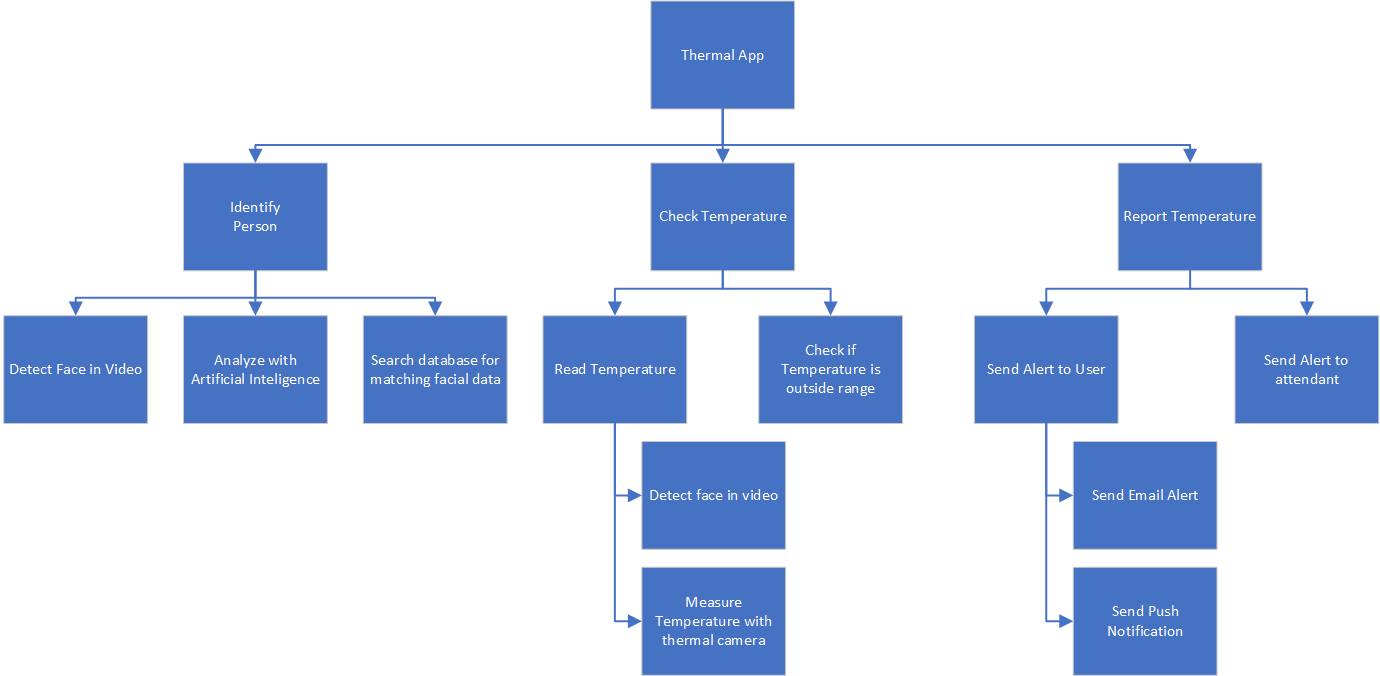
\includegraphics[width=0.8\textwidth]{Function diagram-Thermal App.png}
        \caption{Functional Decomposition Diagram - Thermal scanner}
    \end{figure}
    \begin{figure}[h!]
        \centering
        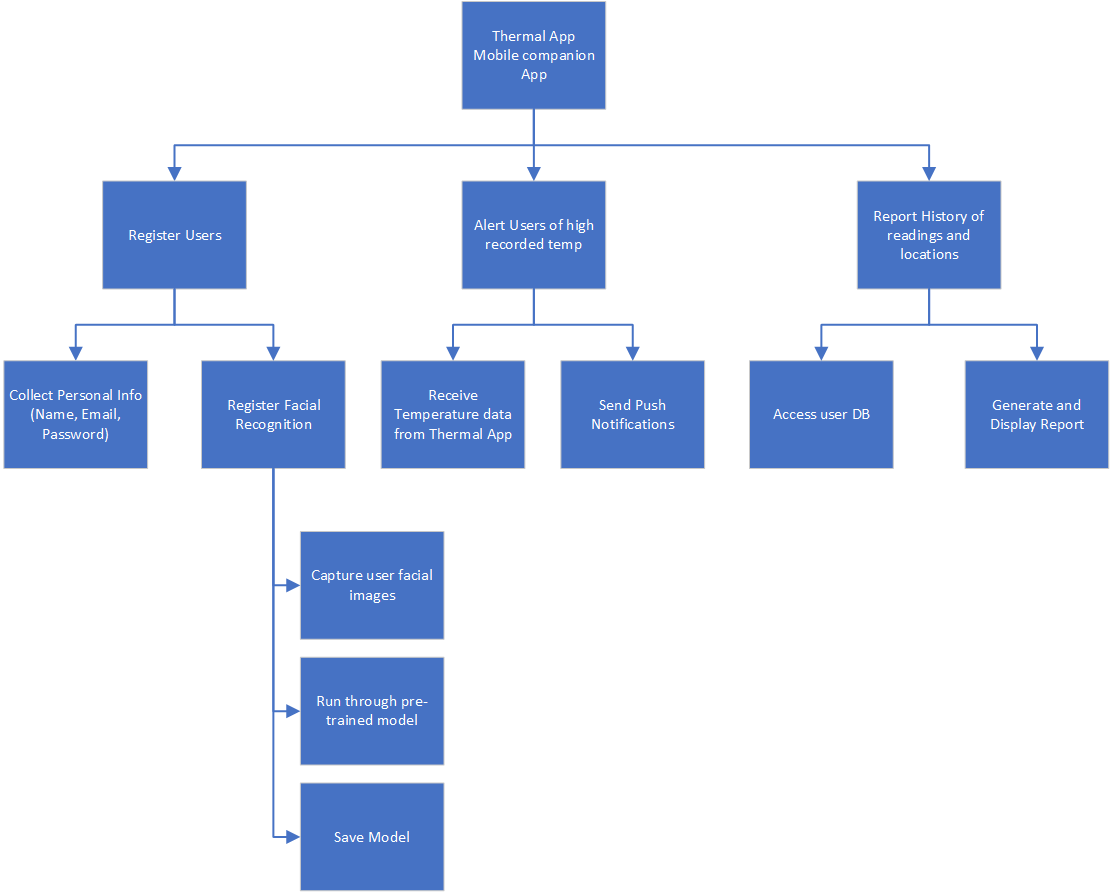
\includegraphics[width=0.8\textwidth]{Function diagram-Mobile Comapanion App.png}
        \caption{Functional Decomposition Diagram - Comapanion App}
    \end{figure}
    \newpage
    \section{Data Flow and Application Structure}
    \begin{figure}[h!]
        \centering
        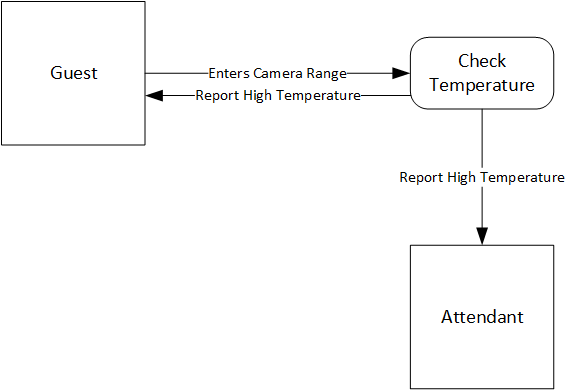
\includegraphics[width=0.8\textwidth]{DFD Top Level.png}
        \caption{Top Level Data Flow Diagram}
    \end{figure}
    \begin{figure}[h!]
        \centering
        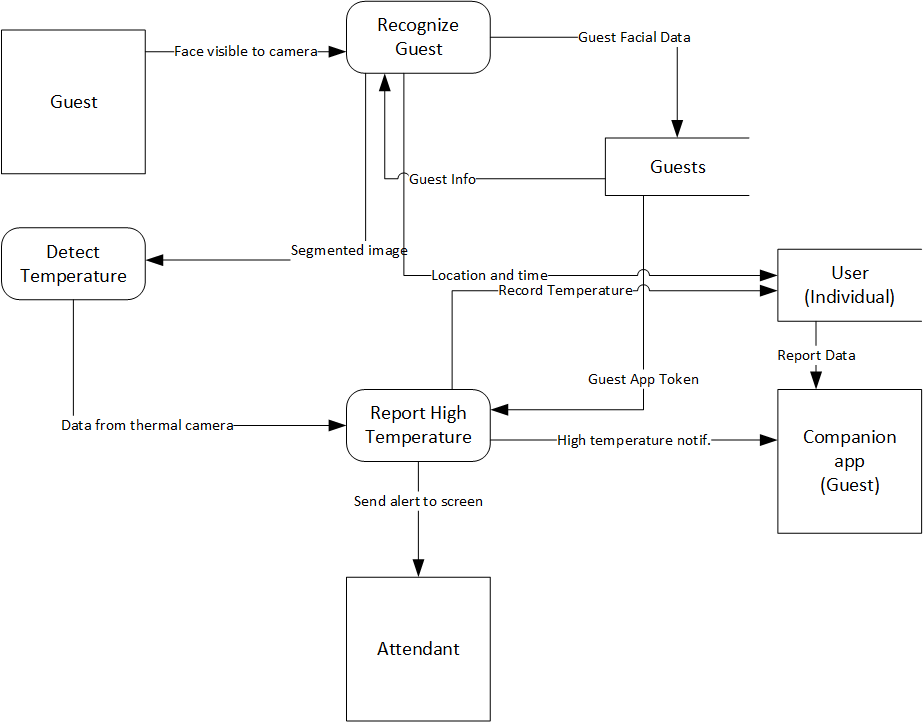
\includegraphics[width=0.8\textwidth]{DFD Level 1.png}
        \caption{Level 1 Data Flow Diagram}
    \end{figure}
    \begin{figure}[h!]
        \centering
        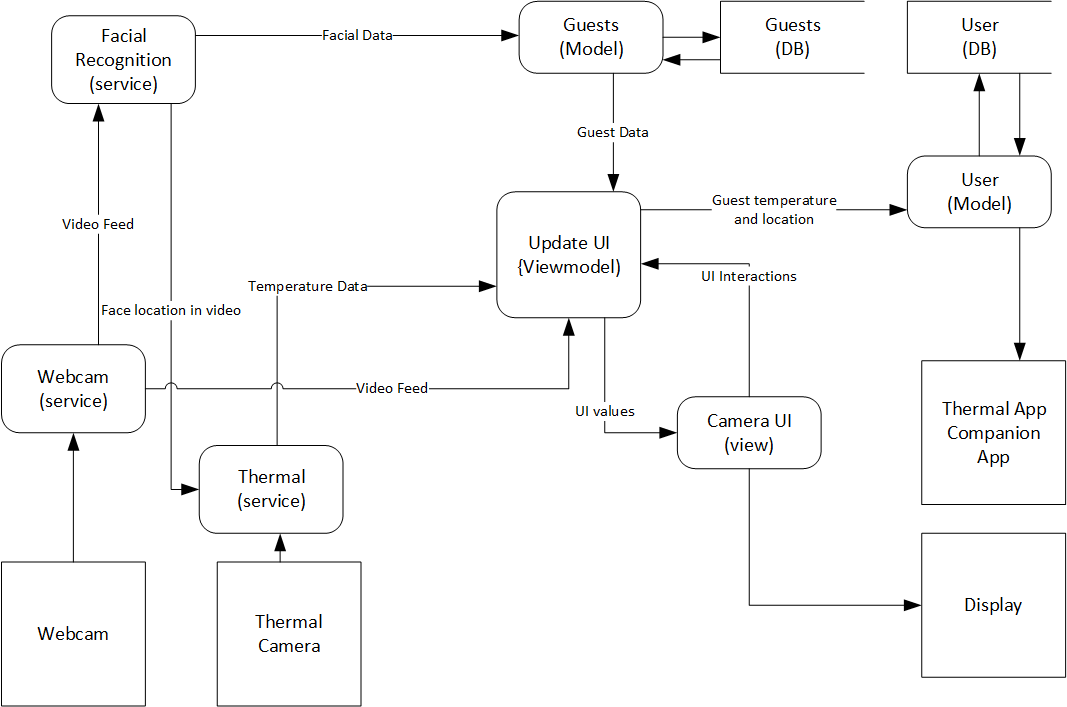
\includegraphics[width=0.8\textwidth]{DFD Level 2.png}
        \caption{Level 2 Data Flow Diagram}
    \end{figure}    
    \section{User Stories and Tasks}
    \begin{table}[ht!]
        \begin{center}
        \begin{tabular}{|>{\centering \arraybackslash}m{3.7cm}|>{\centering \arraybackslash}m{8.5cm}|}
            \hline
            Epic & User Story\\
            \hline
            \multirow{4}{3cm}{Provide facial recognition for user identification and measure user temperature}
                &As a user, I want the system to recognize me in under 2 seconds so I can save time\\\hhline{~-} 
                &As a kiosk attendant, I want to see a confirmation that the user is recognized, for security purposes\\\hhline{~-} 
                &As a kiosk attendant, I want temp measurements to be accurate withing a degree, so I do not have to check extra people/miss people\\\hhline{~-} 
                &As a kiosk attendant, I want the thermal camera to self-calibrate, to avoid the need for time consuming troubleshooting\\
            \hline
            \multirow{3}{3cm}{Provide notifications and reports to users and attendants}
                &As a kiosk attendant, I should be alerted if a registered user is detected with a high temperature to perform a manual temperature check\\\hhline{~-} 
                &As a kiosk attendant, I should be alerted if a person is not recognized as a registered user\\\hhline{~-} 
                &As a user, I should be alerted if my temperature is too high\\\hhline{~-}
            \hline
            \multirow{3}{3cm}{Provide a user onboarding system}
                &As a user, I want to register through a mobile app, for easier remote registration\\\hhline{~-} 
                &As a user, I want to register facial data through the app, so I can skip in person registration\\\hhline{~-} 
                &As a system admin, I want to have control over what information is collected from users and how long the data is stored, to increase security\\\hhline{~-} 
            \hline
        \end{tabular}
        \end{center}
        \caption{Epics and User Stories}
        \label{tab:multicol}
    \end{table}
    \section{Derived tasks and Pseudocode}
    The following tasks and Pseudocode were derived from the user stories listed in Table \ref{tab:multicol}.
    \subsection{Detect faces in video}
    Face detection is used to determine whether a user has entered the view of the camera in order to 
    begin facial recognition and measuring their temperature. This is done using the opencv library in 
    Python.
    \begin{algorithm}
        Read camera stream
        Use OpenCV to detect faces
        Store face pixel array in var
        Apply smoothing and post processing
        Return section array
    \end{algorithm}
    \subsection{Calculate temperature discrepancy and adjust the camera}
    The thermal camera is known to lose accuracy depending on the surrounding temperature and weather 
    conditions. A hot plate will be placed in the vision of the thermal camera and will be used to 
    calibrate it. This will provide more consistent and accurate measurements.
    \begin{algorithm}[caption={Thermal cam calibration.}, label={alg1}]
        timer: every 3 minutes
        on timer firing
            select section of video containing calibration device
            measure temperature
            if measured temperature does not equal set value for temperature
                subtract set from measured temp
                adjust calibration by result
    \end{algorithm}
    \subsection{Measure temperature within the segment of the thermal image that corresponds to the user’s face}
    Once the user's face has been segmented from the video stream, the rgb and thermal images need to be 
    compared and the correct pixels measured for temperature.  Because the resolution is different between the images,
    additional calculations are required. The data from the thermal camera is then returned.
    \begin{algorithm}[caption={Temperatur reading.}, label={alg1}]
        Receive array of pixel data containing face
        Calculate corresponing pixel locations in thermal image
        return thermal readings from those locations
    \end{algorithm}
    \subsection{Check if user is registered}
    Once a face is detected within the cameras vision, the application will use facial detection to 
    store the users facial data and compare it to the facial data already stored in the database to 
    check whether the has been registered through the system.
    \begin{algorithm}[caption={Facial info search.}, label={alg1}]
        Connect to database
        Receive tuple with facial data files
        Loop for length in tuple
            If new data is equivalent to registered data
                User is registered
                Break loop
    \end{algorithm}
    \subsection{Send notifications to user and alerts to screen}
    If a high temperature is detected by the system, the application will send an alert through the 
    screen on the tablet and to a kiosk attendee and the user. The system will also be able to send an 
    alert to the attendee if the user is not registered.
    \begin{algorithm}[caption={Temperature notification}, label={alg1}]
        If high temperature detected
            Display high temperature alert on screen
            Connect to database
            Search for email using user id
            Send message to user email
            Send alert to attendee email
    \end{algorithm}
    \subsection{Compare user temperature to past temps and check for too high temp}
    The application will consider the average temperature of the user by searching through the user’s 
    past scans and taking the average of their temperature history. A limit will be set based on their 
    average temperature. If the user’s temperature passes that limit it will be considered a high 
    temperature.
    \begin{algorithm}[caption={Check user temperature}, label={alg1}]
        Search database for user temperature history using user id
        Receive array with past temperatures
        Initialize counter at 0
        Initialize sum at 0
        Loop for size of array
            Sum is equal to sum plus tuple[counter]
            Average is equal to sum divided by size of array
            Limit is equal to average plus 3 degrees Fahrenheit
            If limit is greater than current temp
                User temp passes
            Else
                User temp fail
    \end{algorithm}
    \subsection{Register facial data through app}
    To reduce the amount of time the user needs to spend registering in person, and to improve registration
    times for large userbases, users will be able to register for the facial recognition from a companion app.  
    Several images will be captured, the algorithm will be trained, and then the images will be deleted and the model
    stored in the database.
    \begin{algorithm}[caption={Register facial data}, label={alg1}]
        App receives access to phone camera
        Use facial detection to detect face
        If face detected
            Take pictures of user
            Convert pictures into facial recognition data files
            Send files to database
    \end{algorithm}
    \subsection{Register users through app}
    Users will be required to provide some identifying piece of information to create an account and eventually register
    facial recognition data
    \begin{algorithm}[caption={Register user data}, label={alg1}]
        User enters identifier
        User enters password
        Form entries are verified for format with regex
        If info matches format
            Create new entry in database
            Store user info
            Send user confirmation email
        if user confirms
            finalize user registration
    \end{algorithm}
    \subsection{Allow admin to control data requested and storage duration}
    User data collected for registration will vary based on use case.  Most use cases will minimize data collected
    to an Employee ID number, but the admin may want to collect more data.  To account for these variations, the 
    application will allow the admin to set what information will be collected and how long the data will be stored.
    \begin{algorithm}[caption={Manage User data settings}, label={alg1}]
        Display list of options with on/off toggles
        Display data storage duration with default value of 1 month
        if at least one option is selected
            enable save button
        on save button clicked
            set user data requirements
            set data expiration time
    \end{algorithm}
    \subsection{Produce reports for organization and users}
    Companies and users will be able to view reports of temperature measured and time/location the data was collected.
    Company reports will list all users for a period of time, including times, location and temperature.  Users will have
    access to similar reports, but only applying to them.
    \begin{algorithm}
        Request time period for reports (Default is 1 month)
        if Company
            query db for users recorded during that period
            display sortable table listing users, locations and temperature
        if User
            query db for users recorded during that period
            display sortable table listing locations and temperature for that user
    \end{algorithm}
    \section{Reflection}
    \subsection{Lessons Learned}
    \paragraph{}
    So far, the team has learned how important it is to communicate and organize tasks, 
    especially between cross disciplinary teams. During the beginning of the project we were a 
    bit confused and overwhelmed because roles and tasks were not clearly defined. Once the 
    team started to document the project and got a better idea of what we had to do it became 
    easier to assign tasks.
    \paragraph{}
    One of the applications that helped us assign and organize tasks was Trello. With Trello we 
    were able to keep track of what everyone is working on and helped us share documentation 
    for the project.
    \subsection{Areas to Improve}
    \paragraph{}
    The team could have done a better job of communicating early in the project and discussing 
    initial requirements such as what programming language we should use. It was not much of 
    an issue because we were still in the early development phase of the project, but it did 
    delay progress somewhat.
    \subsection{Concrete Steps}
    \paragraph{}
    Our team will perform better in the future by communicating more with the Computer Engineering team. We 
    need to meet regularly to know how much progress we have made on the project and discuss 
    implementation and communication of certain functions. This will help to make sure the team 
    is on the same page and the sponsor gets the application they want.
    \paragraph{}
    During the project we have not had a structured development cycle and it has slowed down our 
    progress. We will adopt more of an agile development approach to increase productivity. 
    This will make sure everyone has a task to work on. The team as well as the sponsor will 
    know that progress is being made.
    \subsection{Personal Thoughts}
    \subsubsection{Jose Bastardo}
    \paragraph{}
    A personal weakness of mine that I discovered was being able to communicate with the sponsor 
    and teammates. There were points where I could have asked more questions and discussed 
    things more thoroughly. This possibly comes from some social anxiety, but it has improved 
    as we have moved further into the project.
    \paragraph{}
    A strength that was revealed during this project was my ability to take lead in scheduling 
    and organizing presentations and assignments. I feel like this semester I was able to work 
    on my leadership skills while working on the project and off the project in my own life.
    \subsubsection{Colter Roche}
    \paragraph{}
    Some personal strengths and weaknesses highlighted by this project involved personal 
    struggles with time management and difficulties communicating effectively with the other 
    half of the team.  The change from .NET to Python was not clearly stated in a timely way, 
    so a lot of time was wasted on our end planning the .Net version.  We also did not have 
    weekly meetings with the other half of the team, so the status of the calibration system is 
    mostly unknown.  Going forward, much more rigorous adherence to meeting scheduling and task 
    completion will be necessary.  The trello has only been lightly used, this will need to 
    change for the implementation phase next semester.  
    \paragraph{}
    One positive from the experience has been working closely with Jose to complete reports and 
    presentations, and the process of writing and formatting all the documents.  The move from 
    using word to using \LaTeX for report and documentation writing has been a personal project, 
    and this class was a great opportunity to utilize that skill.
    \section{Conclusion}
    \paragraph{}
    The goals and requirements for this project were fairly straightforward, especially for the 
    CS team: design and implement a UI, implement or otherwise handle facial recognition, and 
    interface with the thermal camera system the CE team is working on.  Unfortunately, 
    communication broke down with the CE team, due to a lack of effort on our part and a 
    (perceived on Colter’s part) lack of professionalism and openness to different solutions.  
    \paragraph{}
    Regardless, we thoroughly planned out the structure and functions of the system and have 
    successfully implemented some of the basic requirements for storing user information.  
    In addition, the programming language for the application has been finalized and work has 
    begun on the UI and the facial recognition.  The progress on the thermal calibration is 
    somewhat in doubt, but at the very least, they have the thermal camera working and are 
    learning the skills they need for image processing with OpenCV.
    \paragraph{}
    Next steps are to continue to investigate and test different options for the facial 
    recognition system.  The code provided from a previous project is essentially two other 
    programs copied and pasted to work together, and the overall process is too slow.  We will 
    attempt to reduce the time by using one of the faster models included with OpenCV.  
    UI implementation should be straightforward, but we have not started any of the 
    designs for the mobile onboarding app.  
    \paragraph{}
    One of the main focuses for next semester’s work 
    will need to be designing the UI and functionality for the app.  The interfacing with the 
    temperature and calibration system will hopefully be straightforward, but the CE team’s 
    status and class structure is unknown since the switch to Python.  Regular inter-team 
    meetings will also need to be scheduled.
    \section{Team Member Participation}
    Participation was split as follows:
    \begin{itemize}
        \item Colter Roche: 50\%
        \item Jose Bastardo: 50\%
    \end{itemize}
\end{document}